\documentclass[UTF8,a4paper,11pt,fontset=fandol]{ctexart}
\usepackage{geometry}
\geometry{margin=2.2cm}
\usepackage{amsmath,amssymb,longtable,booktabs,array,hyperref,xcolor,enumitem,graphicx,float}
\hypersetup{colorlinks=true,linkcolor=blue,urlcolor=blue}
\setlist[itemize]{leftmargin=1.3em,itemsep=0.2em}
\definecolor{notegray}{RGB}{246,248,251}
\title{P04. Real-time Cooperative Vehicle Coordination at Unsignalized Road Intersections\\中英双语博士精读笔记}
\author{Jiping Luo; Tingting Zhang; Rui Hao; Donglin Li; Chunsheng Chen; Zhenyu Na; Qinyu Zhang}
\date{2023 · IEEE Transactions on Intelligent Transportation Systems}
\begin{document}
\maketitle

\noindent\textbf{Theme / 主题：} DRL cooperative trajectory optimization\\
\textbf{Method family / 方法族：} TD3 deep reinforcement learning for coordination / TD3 深度强化学习协同控制\\
\textbf{PDF pages / 页数：} 15 \quad
\textbf{Relevance / 相关度：} 91/100\\
\textbf{Source / 来源：} \url{https://arxiv.org/abs/2205.01278}

\section{论文全景速览与核心贡献 / High-Level Overview \& Core Contributions}
\subsection{研究背景与痛点 / Background \& Pain Points}
这篇论文位于“DRL cooperative trajectory optimization”方向。对你的 JSSP-based Intersection Management 课题，它回答的是高层调度、低层轨迹平滑、安全过滤或真实验证中的一个关键子问题：如何让车辆在路口少停、少冲突、少能耗，同时保持在线可执行。

The paper belongs to the theme of DRL cooperative trajectory optimization. For a JSSP-based intersection-management thesis, it illuminates one of the key layers: scheduling, smoothing, safety filtering, or real-world validation.

\textbf{Pain point / 痛点：} Centralized control-authority handoff and DRL policy behavior may be difficult to certify in mixed traffic.

\subsection{核心科学问题 / Core Scientific Question}
能否用连续动作深度强化学习直接学习无信号交叉口的实时协同轨迹控制策略？

Can continuous-control deep reinforcement learning learn real-time cooperative trajectories for unsignalized intersections?

\subsection{科学贡献 / Scientific Contributions}
\begin{itemize}
\item 方法贡献 (method contribution)：Formulates unified cooperative trajectory optimization for unsignalized intersections and solves the sequential decision problem with TD3.
\item 安全/避碰贡献 (safety contribution)：Safety and long-term stability constraints are embedded in the cooperative trajectory optimization framework.
\item 平滑/停止避免贡献 (smoothing contribution)：Optimizes throughput and continuous flow, reducing delay compared with conservative coordination.
\item 创新力度评判 (reviewer judgement)：较强应用创新：将 TD3 用于统一协同轨迹优化并强调毫秒级推理，但可验证安全仍是短板。
\end{itemize}


\subsection{核心概念对照 / Core Concepts}
\begin{longtable}{p{0.24\linewidth}p{0.28\linewidth}p{0.40\linewidth}}
\toprule
中文概念 & English Concept & Role / 学术作用\\
\midrule
自动交叉口管理 & Autonomous Intersection Management & 把信号控制替换为车辆级调度与控制。 \\
轨迹平滑 & Trajectory Smoothing & 减少急加减速、停车和能耗峰值。 \\
安全约束 & Safety Constraints & 把碰撞风险写成距离、时间间隔或屏障函数。 \\
TD3 deep reinforcement learning for coordination & TD3 深度强化学习协同控制 & 该论文的核心方法族。 \\
\bottomrule
\end{longtable}

\section{教材式学习路径与关键截图 / Textbook-Style Study Path \& PDF Snapshots}
\subsection{学习路径 / Study Path}
\begin{itemize}
\item 第一遍先读首页截图、摘要与引言，确认研究问题和场景假设。
\item 第二遍沿着技术路线图复现模型变量、约束和求解器输入输出。
\item 第三遍逐节阅读 section deep reading，对照 PDF 截图检查公式、图表和实验。
\item 第四遍只站在审稿人视角重读实验，判断 baseline、公平性、消融和鲁棒性。
\item 最后把博士 checklist 写成自己的复现实验或论文拓展计划。
\end{itemize}


\subsection{博士阅读 Checklist / Doctoral Reading Checklist}
\begin{itemize}
\item 能否独立重写核心公式：MDP 目标与 TD3 策略优化 / MDP objective and TD3 policy optimization，并解释每个符号的物理意义？
\item 能否画出输入-模型-算法-控制-验证的数据流图？
\item 能否指出至少两个强假设，并说明它们在真实交通中何时失效？
\item 能否复述实验基准是否公平，指标是否覆盖效率、安全、能耗和计算时间？
\item 能否提出一个与自己 JSSP/RL/smoother 课题直接相连的拓展实验？
\end{itemize}


\subsection{关键截图讲解 / PDF Snapshot Explanation}
Screenshots are selected anchors from the local PDFs for study and parallel reading. They do not replace the original paper.

\begin{figure}[H]
\centering

\includegraphics[width=0.92\linewidth]{../../assets/P04_luo2023realtime/01_title_and_abstract_p1.jpg}
\caption{首页与摘要 / Title and abstract page (p.1, full\_page). 这张截图用于把笔记中的抽象概念拉回原论文页面，便于你平行阅读原文、公式、图表和实验设置。 与当前课题的连接：Shows why learned policies are attractive for online intersection coordination but need a structured safety/smoothing interface.}
\end{figure}

\begin{figure}[H]
\centering

\includegraphics[width=0.92\linewidth]{../../assets/P04_luo2023realtime/02_modeling_or_problem_setup_p2.jpg}
\caption{建模或问题设定页 / Modeling or problem-setup page (p.2, full\_page). 这张截图用于把笔记中的抽象概念拉回原论文页面，便于你平行阅读原文、公式、图表和实验设置。 与当前课题的连接：Shows why learned policies are attractive for online intersection coordination but need a structured safety/smoothing interface.}
\end{figure}

\begin{figure}[H]
\centering
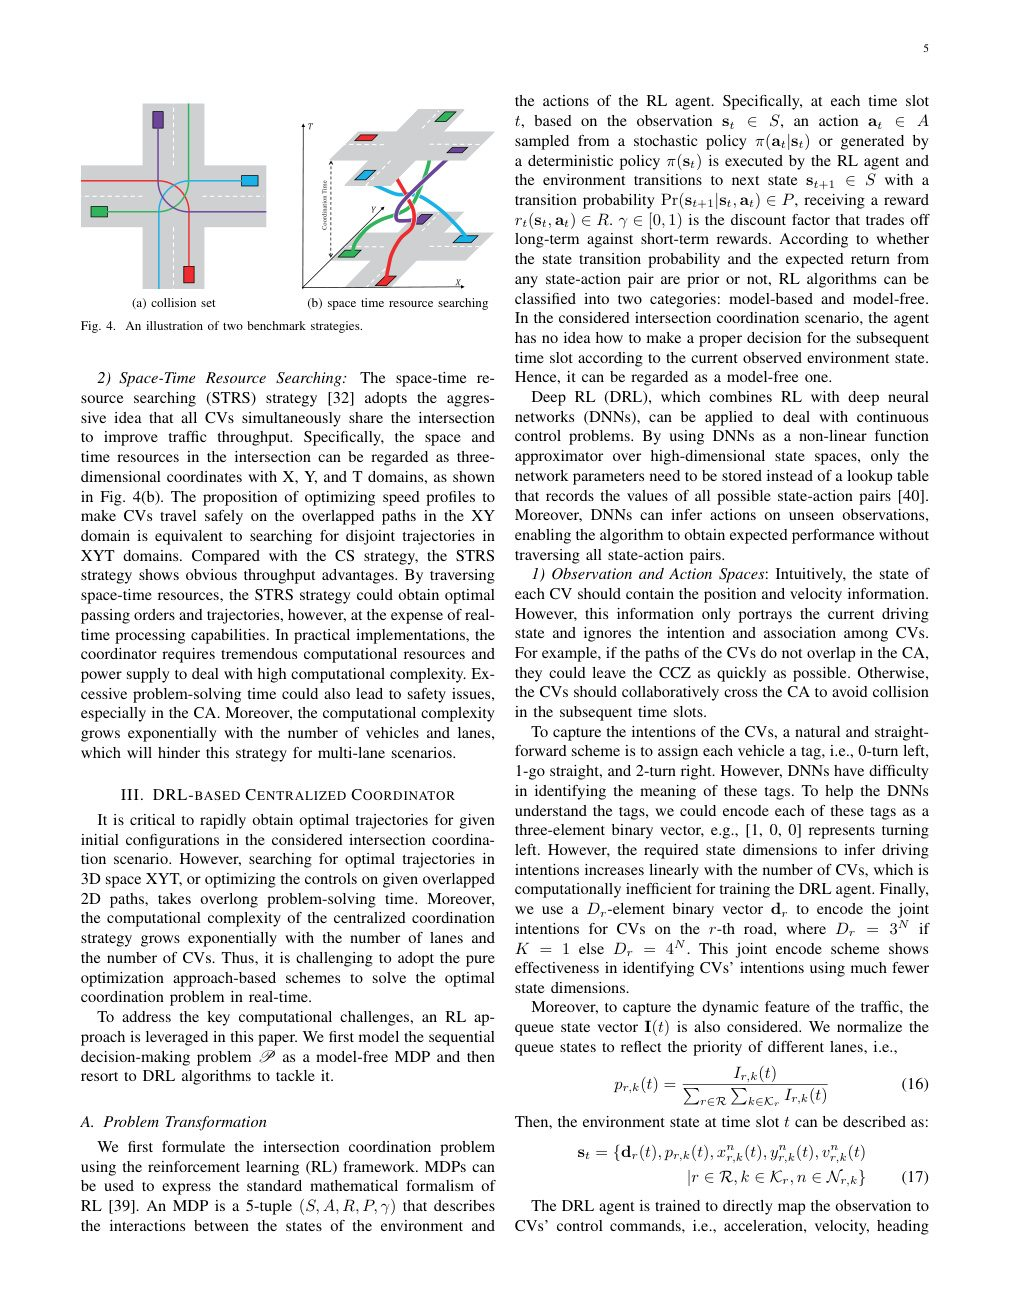
\includegraphics[width=0.92\linewidth]{../../assets/P04_luo2023realtime/03_core_method_or_algorithm_p5.jpg}
\caption{核心方法或算法页 / Core method or algorithm page (p.5, full\_page). 这张截图用于把笔记中的抽象概念拉回原论文页面，便于你平行阅读原文、公式、图表和实验设置。 与当前课题的连接：Shows why learned policies are attractive for online intersection coordination but need a structured safety/smoothing interface.}
\end{figure}

\begin{figure}[H]
\centering
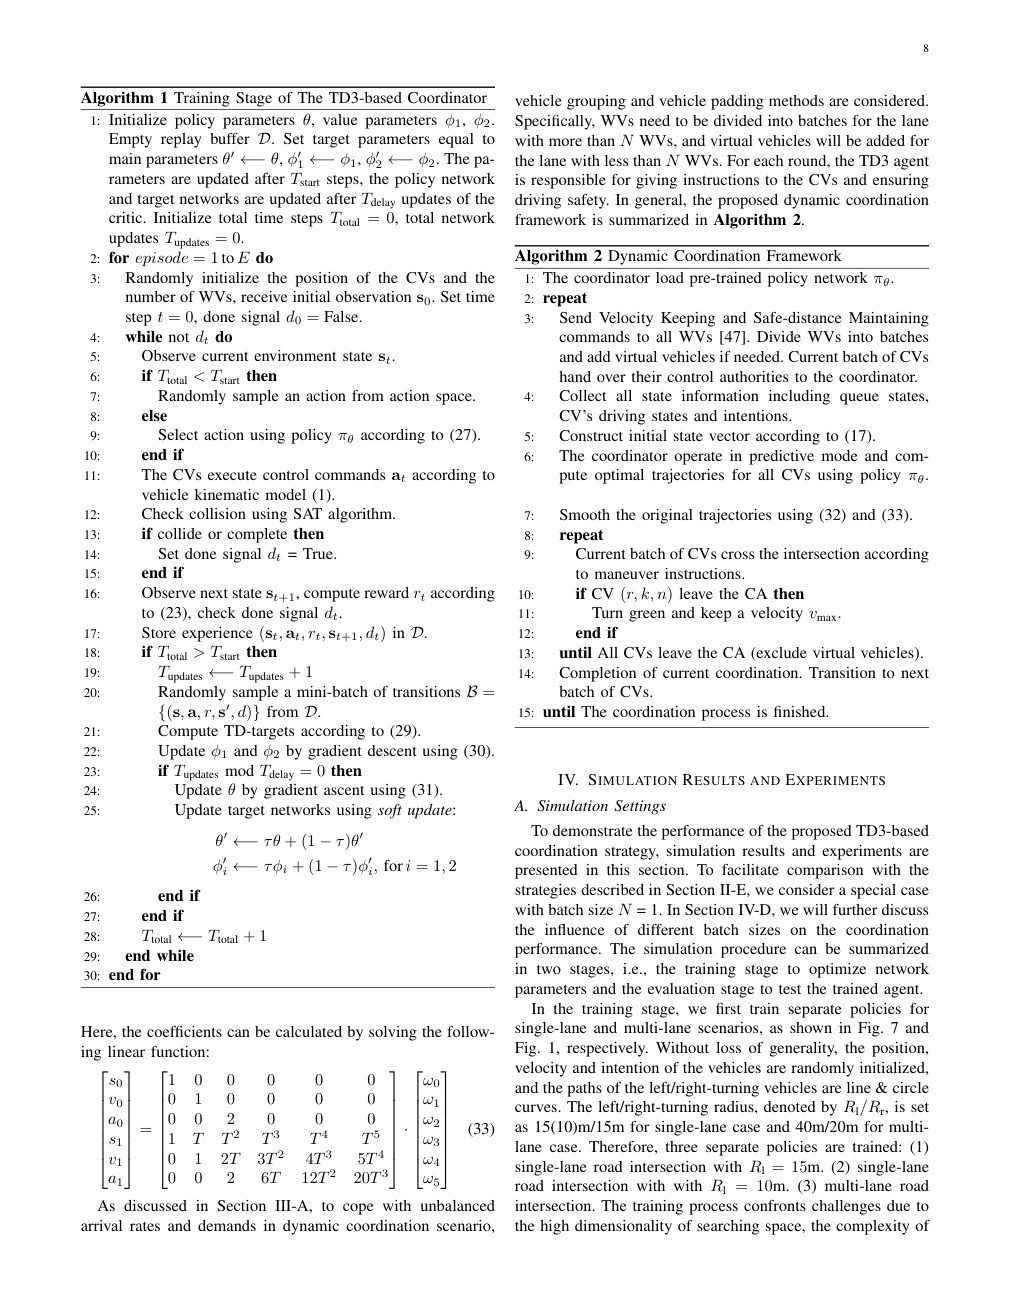
\includegraphics[width=0.92\linewidth]{../../assets/P04_luo2023realtime/04_experiments_or_results_p8.jpg}
\caption{实验或结果页 / Experiments or results page (p.8, full\_page). 这张截图用于把笔记中的抽象概念拉回原论文页面，便于你平行阅读原文、公式、图表和实验设置。 与当前课题的连接：Shows why learned policies are attractive for online intersection coordination but need a structured safety/smoothing interface.}
\end{figure}

\begin{figure}[H]
\centering

\includegraphics[width=0.92\linewidth]{../../assets/P04_luo2023realtime/05_conclusion_or_limitations_p13.jpg}
\caption{结论或局限页 / Conclusion or limitations page (p.13, full\_page). 这张截图用于把笔记中的抽象概念拉回原论文页面，便于你平行阅读原文、公式、图表和实验设置。 与当前课题的连接：Shows why learned policies are attractive for online intersection coordination but need a structured safety/smoothing interface.}
\end{figure}


\section{章节精读与逐段导读 / Section-by-Section Deep Reading \& Walkthrough}
\subsection*{p.1 I. INTRODUCTION}
\textbf{章节目标 / Learning goal：} 建立研究动机：为什么传统信号控制、FCFS 或单车控制不足以处理该论文关注的交叉口协同问题。

Understand why the paper needs a new coordination method rather than a standard signal, FCFS, or single-vehicle controller.

\textbf{关键论点 / Key argument：} 这一部分通常把痛点落到 DRL cooperative trajectory optimization：既要提高效率，又要保持安全与在线可执行。

\textbf{技术焦点 / Technical focus：} 精读时标出作者批判的 baseline、场景假设、交通参与者类型和隐含优化目标。

\textbf{审稿追问 / Reviewer question：} 作者指出的痛点是否真的需要新方法，还是可以由更强的优化器/更保守规则解决？

\subsection*{p.2 II. S YSTEM MODEL}
\textbf{章节目标 / Learning goal：} 把自然语言交通问题压缩为变量、状态、约束、目标函数或图结构。

Translate the traffic problem into variables, states, constraints, objectives, or graph relations.

\textbf{关键论点 / Key argument：} 本节是复现论文的核心入口，应与公式“MDP 目标与 TD3 策略优化 / MDP objective and TD3 policy optimization”一起读。

\textbf{技术焦点 / Technical focus：} 逐项检查车辆状态、冲突关系、控制输入、时间/空间索引和安全阈值是否定义完整。

\textbf{审稿追问 / Reviewer question：} 这些建模假设在混合交通、通信延迟、感知误差和高密度车流下是否仍成立？

\subsection*{p.3 3. The road region occupied by the vehicle is defined by a two-}
\textbf{章节目标 / Learning goal：} 承接前后章节，补充局部定义、案例或实现细节。

Recover implementation details needed for reproduction.

\textbf{关键论点 / Key argument：} 这类章节常常不是主贡献，但决定你能否真正复现方法。

\textbf{技术焦点 / Technical focus：} 检查它是否给出了参数、伪代码、场景划分或实现细节。

\textbf{审稿追问 / Reviewer question：} 跳过该节会不会导致公式或实验无法复现？

\subsection*{p.5 III. DRL- BASED CENTRALIZED COORDINATOR}
\textbf{章节目标 / Learning goal：} 解释算法如何把模型转化为可执行决策，并说明在线运行机制。

Trace how the paper turns the model into executable online decisions.

\textbf{关键论点 / Key argument：} 将协同控制表述为连续动作 MDP，TD3 使用双评论家取最小值、延迟 actor 更新和目标策略平滑来提升稳定性。在线执行时只需前向传播策略网络，因而推理很快。

\textbf{技术焦点 / Technical focus：} 画出输入、核心求解器、输出和安全检查接口，明确哪些步骤是优化、哪些是规则、哪些是学习。

\textbf{审稿追问 / Reviewer question：} 若算法某一步失败，论文有没有 fallback、重规划或安全过滤机制？

\subsection*{p.8 1 T T 2 T 3 T 4 T 5}
\textbf{章节目标 / Learning goal：} 承接前后章节，补充局部定义、案例或实现细节。

Recover implementation details needed for reproduction.

\textbf{关键论点 / Key argument：} 这类章节常常不是主贡献，但决定你能否真正复现方法。

\textbf{技术焦点 / Technical focus：} 检查它是否给出了参数、伪代码、场景划分或实现细节。

\textbf{审稿追问 / Reviewer question：} 跳过该节会不会导致公式或实验无法复现？

\subsection*{p.8 IV. SIMULATION RESULTS AND EXPERIMENTS}
\textbf{章节目标 / Learning goal：} 验证方法是否在公平基准下改善效率、安全、能耗或计算时间。

Check whether the claimed improvements are supported by fair baselines and meaningful metrics.

\textbf{关键论点 / Key argument：} 实验应与论文声称的贡献闭环：Simulation and practical experiments; authors report millisecond-scale computation and scalability with lane count.

\textbf{技术焦点 / Technical focus：} 重点追踪指标：平均通行时间、吞吐量、延误、速度波动、碰撞/冲突次数和在线计算耗时。 同时检查仿真平台、交通需求和随机性设置。

\textbf{审稿追问 / Reviewer question：} 实验是否只展示平均收益，还是覆盖了高密度、异常扰动和失败案例？

\subsection*{p.13 V. CONCLUSION}
\textbf{章节目标 / Learning goal：} 提炼作者承认的边界，并把它转化为博士课题的可拓展问题。

Convert acknowledged boundaries into research opportunities.

\textbf{关键论点 / Key argument：} 结论不只是总结结果，更是观察作者没有解决什么的窗口。

\textbf{技术焦点 / Technical focus：} 把 future work 与前文假设逐一对应，寻找可发表的补强点。

\textbf{审稿追问 / Reviewer question：} 如果我是审稿人，我会要求补哪一个实验、定理或消融？


\subsection{逐段式导读 / Paragraph-Level Walkthrough}
\paragraph{Opening motivation / 开篇动机段}先把作者的痛点翻译成一句博士问题：能否用连续动作深度强化学习直接学习无信号交叉口的实时协同轨迹控制策略？ 读这一段时不要急着接受动机，要追问传统 FCFS、信号灯或保守 MPC 为什么不足。

Turn the opening motivation into one doctoral-level question and test whether the paper truly needs a new method.

\paragraph{Assumption and setting / 假设与场景段}把车辆类型、通信条件、路口类型和动力学假设列成表。该文的关键边界包括：训练环境覆盖了测试场景的关键交通分布。；中心协调器能获得足够完整的车辆状态。；奖励函数能充分惩罚碰撞、剧烈加减速和低效率。

List vehicle type, communication, intersection setting, and dynamics assumptions before reading the equations.

\paragraph{Model and notation / 模型与符号段}围绕核心公式“MDP 目标与 TD3 策略优化 / MDP objective and TD3 policy optimization”复写符号表，确认每个变量是决策变量、状态变量、参数还是约束阈值。

Rewrite the symbol table around the core formulation and classify variables as states, decisions, parameters, or constraints.

\paragraph{Algorithm mechanism / 算法机制段}把算法读成一条数据流：输入交通状态，执行 Formulates unified cooperative trajectory optimization for unsignalized intersections and solves the sequential decision problem with TD3.，输出可执行通行/控制决策，并检查安全接口。

Read the algorithm as a dataflow from traffic state to executable sequence/control decision, with explicit safety interfaces.

\paragraph{Experiment and evidence / 实验证据段}不要只看作者报告的提升，要检查基准、公平性和指标。本文验证描述为：Simulation and practical experiments; authors report millisecond-scale computation and scalability with lane count.

Go beyond reported gains and inspect baselines, fairness, metrics, and computation time.

\paragraph{Reviewer synthesis / 审稿式总结段}最后把贡献拆成可发表与需补强两部分。对你课题最直接的用途是：Shows why learned policies are attractive for online intersection coordination but need a structured safety/smoothing interface.

Separate publishable contribution from missing evidence, then connect the result to your own thesis architecture.


\section{技术路线图与贡献量评估 / Technical Route \& Contribution Matrix}
\begin{longtable}{p{0.08\linewidth}p{0.24\linewidth}p{0.58\linewidth}}
\toprule
Step & Stage / 阶段 & Content / 内容\\
\midrule
1 & 输入 / Input & 车辆状态、路径/车道、交通需求、信号或协同信息。 \\
2 & 建模 / Modeling & MDP 目标与 TD3 策略优化 / MDP objective and TD3 policy optimization \\
3 & 核心求解 / Core solver & Formulates unified cooperative trajectory optimization for unsignalized intersections and solves the sequential decision problem with TD3. \\
4 & 安全接口 / Safety interface & Safety and long-term stability constraints are embedded in the cooperative trajectory optimization framework. \\
5 & 平滑与效率 / Smoothing and efficiency & Optimizes throughput and continuous flow, reducing delay compared with conservative coordination. \\
6 & 验证 / Validation & Simulation and practical experiments; authors report millisecond-scale computation and scalability with lane count. \\
\bottomrule
\end{longtable}

\begin{longtable}{p{0.34\linewidth}p{0.14\linewidth}p{0.42\linewidth}}
\toprule
Dimension / 维度 & Score & Comment / 评语\\
\midrule
理论贡献 / Theoretical contribution & 3/5 & MDP 目标与 TD3 策略优化 / MDP objective and TD3 policy optimization \\
算法贡献 / Algorithmic contribution & 4/5 & Formulates unified cooperative trajectory optimization for unsignalized intersections and solves the sequential decision problem with TD3. \\
实验贡献 / Experimental contribution & 3/5 & Simulation and practical experiments; authors report millisecond-scale computation and scalability with lane count. \\
工程贡献 / Engineering contribution & 3/5 & Safety and long-term stability constraints are embedded in the cooperative trajectory optimization framework. \\
博士课题价值 / PhD relevance & 5/5 & Shows why learned policies are attractive for online intersection coordination but need a structured safety/smoothing interface. \\
\bottomrule
\end{longtable}

\section{理论方法论深度解构 / Methodology \& Theoretical Framework}
\subsection{问题数学建模 / Mathematical Formulation}
\textbf{MDP 目标与 TD3 策略优化 / MDP objective and TD3 policy optimization}
\[
\max_{\pi_\theta}\; \mathbb{E}\left[\sum_{t=0}^{T}\gamma^t r(s_t,a_t)\right],\quad a_t=\pi_\theta(s_t),\quad y=r+\gamma\min_{k=1,2}Q_{\phi_k}(s',\pi_{\bar\theta}(s'))
\]
\begin{longtable}{p{0.16\linewidth}p{0.25\linewidth}p{0.25\linewidth}p{0.25\linewidth}}
\toprule
Symbol / 符号 & 含义 & Meaning & Role / 建模作用\\
\midrule
s\_t & 协同状态 & cooperative state & 包含车辆位置、速度和交互信息 \\
a\_t & 连续控制动作 & continuous action & 通常对应加速度或轨迹控制量 \\
r & 奖励函数 & reward & 平衡效率、安全和舒适性 \\
gamma & 折扣因子 & discount factor & 决定长期收益权重 \\
Q\_phi & 评论家网络 & critic network & 估计动作价值并抑制过估计 \\
\bottomrule
\end{longtable}

\subsection{核心算法架构 / Core Algorithm Layout}
将协同控制表述为连续动作 MDP，TD3 使用双评论家取最小值、延迟 actor 更新和目标策略平滑来提升稳定性。在线执行时只需前向传播策略网络，因而推理很快。

The cooperative control problem is cast as a continuous-action MDP; TD3 uses clipped double-Q learning, delayed policy updates, and target smoothing for stable training and fast inference.

\subsection{收敛性、稳定性或实时性 / Convergence, Stability, Real-Time Feasibility}
训练稳定性来自 TD3 机制而非形式化安全证明；实时性来自神经网络推理。若状态分布偏移，策略可能给出未认证动作。

TD3 improves learning stability, but safety remains empirical unless wrapped by a constraint layer or safety filter.

\subsection{潜在假设与边界条件 / Assumptions \& Boundary Conditions}
\begin{itemize}
\item 训练环境覆盖了测试场景的关键交通分布。
\item 中心协调器能获得足够完整的车辆状态。
\item 奖励函数能充分惩罚碰撞、剧烈加减速和低效率。
\end{itemize}


\section{实验验证与结果评判 / Experimental Validation \& Result Evaluation}
\textbf{Baselines \& Environment / 基准与环境：} 传统协同控制、非协同策略、FCFS/规则控制和其他深度强化学习控制器。

\textbf{Validation / 验证：} Simulation and practical experiments; authors report millisecond-scale computation and scalability with lane count.

\textbf{Metrics / 指标：} 平均通行时间、吞吐量、延误、速度波动、碰撞/冲突次数和在线计算耗时。

\textbf{Ablation / 消融：} 应检查奖励项、双评论家、目标策略平滑和安全惩罚各自贡献；若缺少这些消融，审稿时会质疑可解释性。

\textbf{Reviewer reading / 审稿式阅读提醒：} 阅读实验时不要只看平均值；应检查交通密度、车流方向、随机种子、失败案例和计算耗时。For doctoral reading, inspect density regimes, demand patterns, random seeds, failure cases, and computation time rather than only mean improvements.

\subsection{图表阅读线索 / Figure and Table Reading Cues}
PDF extraction detected approximately 55 figure references and 1 table references. Exact captions remain in the original PDF; the bilingual cues below tell you what to inspect first.

\begin{longtable}{p{0.24\linewidth}p{0.30\linewidth}p{0.36\linewidth}}
\toprule
图表名称 & Figure/Table Name & Reading focus / 阅读重点\\
\midrule
系统框架图 & system framework diagram & 先确认输入、决策层、控制层和安全约束之间的数据流。 \\
策略网络/训练流程图 & policy-network or training-pipeline diagram & 检查状态、动作、奖励、经验回放和安全惩罚是否闭环一致。 \\
实验指标对比图表 & experimental metric comparison plots/tables & 重点看平均值之外的密度变化、失败场景、计算时间和方差。 \\
\bottomrule
\end{longtable}

\section{审稿人视角：批判性思考与未来方向 / Critical Thinking \& Future Directions}
\subsection{论文局限性 / Limitations \& Weaknesses}
\begin{itemize}
\item 学习策略难以给出严格安全证书。
\item 仿真到真实 (sim-to-real) 分布偏移可能显著。
\item 集中式状态采集和控制权切换在工程落地中成本较高。
\end{itemize}


\subsection{博士课题拓展点 / Research Extensions for PhD}
\begin{itemize}
\item 在 TD3 actor 后接 CBF/MPC safety shield，形成 learn-then-filter 架构。
\item 把 JSSP 调度作为高层离散动作，TD3 只负责连续轨迹平滑。
\item 用离线强化学习或保守 Q 学习降低在线探索风险。
\end{itemize}


\subsection{如何服务当前课题 / Use in This Project}
Shows why learned policies are attractive for online intersection coordination but need a structured safety/smoothing interface.

\section{交互式可视化与 PDF 排版蓝图 / Interactive Visualization \& PDF Layout Blueprint}
\textbf{动态参数 / Parameter：} 安全奖励权重 / Safety reward weight, range [0.1, 5.0] .

权重提高通常降低冲突风险，但过高会造成保守减速和吞吐下降。

Higher safety reward reduces conflicts but may make the policy conservative.

\subsection{HTML 结构化布局建议 / HTML Structuring}
\begin{itemize}
\item 顶部固定 metadata bar：题名、作者、年份、主题、PDF 页数。
\item 左侧目录/section navigator，右侧为五大精读模块。
\item 公式卡片使用 <pre> 或 LaTeX block，紧跟符号表。
\item 审稿人批注用 reviewer-note block，博士拓展用 research-idea list。
\item 交互参数用 input[type=range] + canvas 曲线，打印 PDF 时隐藏交互控件但保留解释。
\end{itemize}


\section{来源锚点与逐节阅读路径 / Source Anchors \& Section-by-Section Reading Map}
\begin{longtable}{p{0.14\linewidth}p{0.76\linewidth}}
\toprule
Page & Extracted heading\\
\midrule
p.1 & I. INTRODUCTION \\
p.2 & II. S YSTEM MODEL \\
p.8 & IV. SIMULATION RESULTS AND EXPERIMENTS \\
\bottomrule
\end{longtable}

\paragraph{p.1 I. INTRODUCTION}定位问题背景、研究缺口和为什么现有保守/非协同方法不足。 / Frames the motivation, research gap, and limits of conservative or non-cooperative methods.

\paragraph{p.2 II. S YSTEM MODEL}把交通交互转写为状态、约束、目标或图结构，是精读时最应复现的部分。 / Defines states, constraints, objectives, or graph structures; this is the section to reproduce carefully.

\paragraph{p.3 3. The road region occupied by the vehicle is defined by a two-}作为局部论证段落阅读，关注它如何服务主问题。 / Read as a local argument and ask how it supports the main question.

\paragraph{p.5 III. DRL- BASED CENTRALIZED COORDINATOR}作为局部论证段落阅读，关注它如何服务主问题。 / Read as a local argument and ask how it supports the main question.

\paragraph{p.8 1 T T 2 T 3 T 4 T 5}作为局部论证段落阅读，关注它如何服务主问题。 / Read as a local argument and ask how it supports the main question.

\paragraph{p.8 IV. SIMULATION RESULTS AND EXPERIMENTS}检验方法是否真的改善效率、安全或能耗；要关注基准是否公平。 / Tests efficiency, safety, or energy claims; inspect whether baselines are fair.

\paragraph{p.13 V. CONCLUSION}总结贡献和未来方向，也常暴露作者承认的边界条件。 / Summarizes contributions and often reveals author-recognized boundaries.


\end{document}
